\documentclass{report}

\usepackage{graphicx}
% \usepackage{subfigure}
\usepackage{caption}
\usepackage{subcaption}

\usepackage{algorithm}
\usepackage{algpseudocode}

\title{Random Walks course project: Simulated Annealing Algorithm for Graph Coloring}

\author{
  R\'oger Berm\'udez Chac\'on\\EPFL
  \and
  Victor Kristof\\EPFL
  \and
  Merlin Nimier-David\\EPFL
}

\begin{document}
  \maketitle

  % -----------------------------------------------------------------------------------
  \section*{Problem statement}
  \paragraph{Proper q-colorings}
  TODO: Define the problem. Show how the problem is posed as an optimization (cost, etc).

  \paragraph{Input data}
  TODO: Describe construction of the random graph. Describe parameters. Show examples for different density parameters.

  \begin{figure}
      \centering
      \begin{subfigure}[t]{3.8cm}
        \centering
        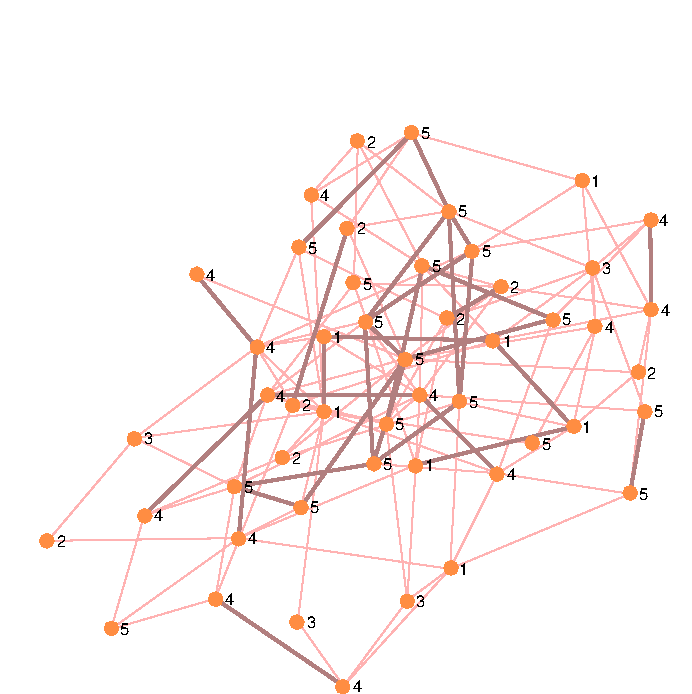
\includegraphics[width=3.8cm]{figures/random-graph-50-5-5.pdf}
        \caption{$c = 5$}\label{fig:1a}
      \end{subfigure}
      \begin{subfigure}[t]{3.8cm}
        \centering
        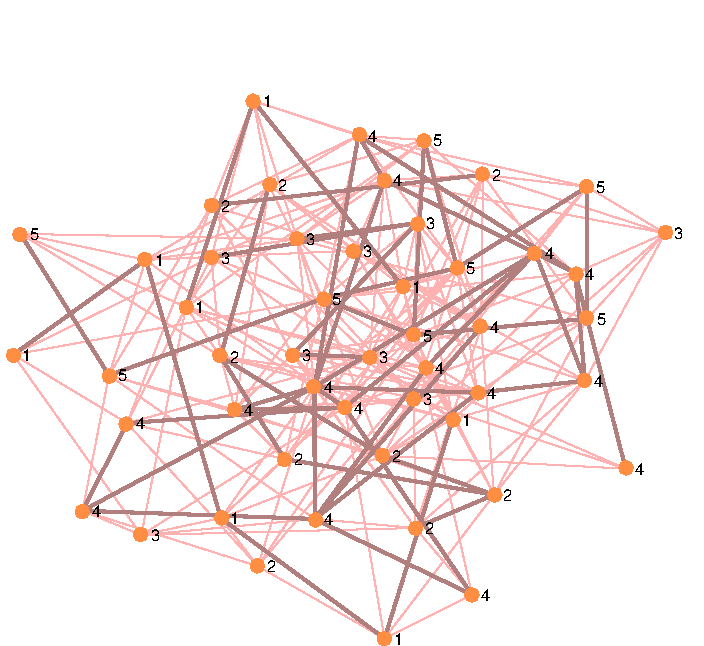
\includegraphics[width=3.8cm]{figures/random-graph-50-10-5.pdf}
        \caption{$c = 10$}\label{fig:1a}
      \end{subfigure}
      \quad
      \begin{subfigure}[t]{3.8cm}
        \centering
        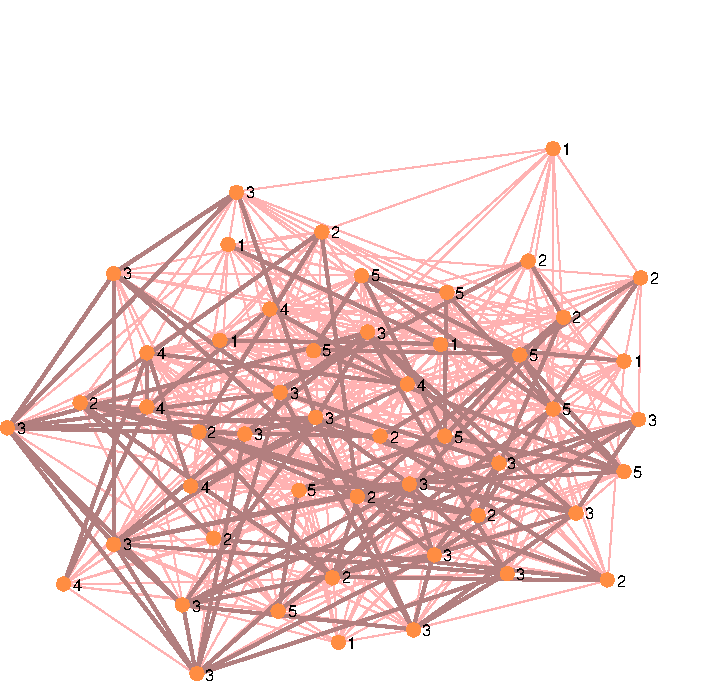
\includegraphics[width=3.8cm]{figures/random-graph-50-20-5.pdf}
        \caption{$c = 20$}\label{fig:1b}
      \end{subfigure}

    \label{Fig:random-graph-examples}
    \caption{Examples of Erd\"{o}s-R\'{e}nyi random graphs for different values of the density parameter $c$. We also visualize an initial random coloring: edges in bold are in conflict, as they have the same color.}
  \end{figure}

  % -----------------------------------------------------------------------------------
  \section*{Metropolis solution}
  \paragraph{TODO} Describe how the optimization can be solved using Metropolis. Explain why we're convinced it will converge if there is a proper coloring.

  % -----------------------------------------------------------------------------------
  \section*{Simulated annealing}
  \paragraph{TODO} Describe the intuition behind the ``temperature''. Define what's a schedule.

  % -----------------------------------------------------------------------------------
  \section*{Results}
  \paragraph{Implementation details}
  TODO: Efficient implementations for generating the graph, transitioning, etc. Give some number to describe algorithm's performance (e.g. average time / iteration).

  \paragraph{Experiments}
  TODO: Explain the different schedules that we tried. Give specific numbers for each parameter (min / max temperature used, starting point, etc). Show results plot for each. Pick the best one and give intuition as to why it performs better than the others.

  \begin{figure}
    \begin{center}
      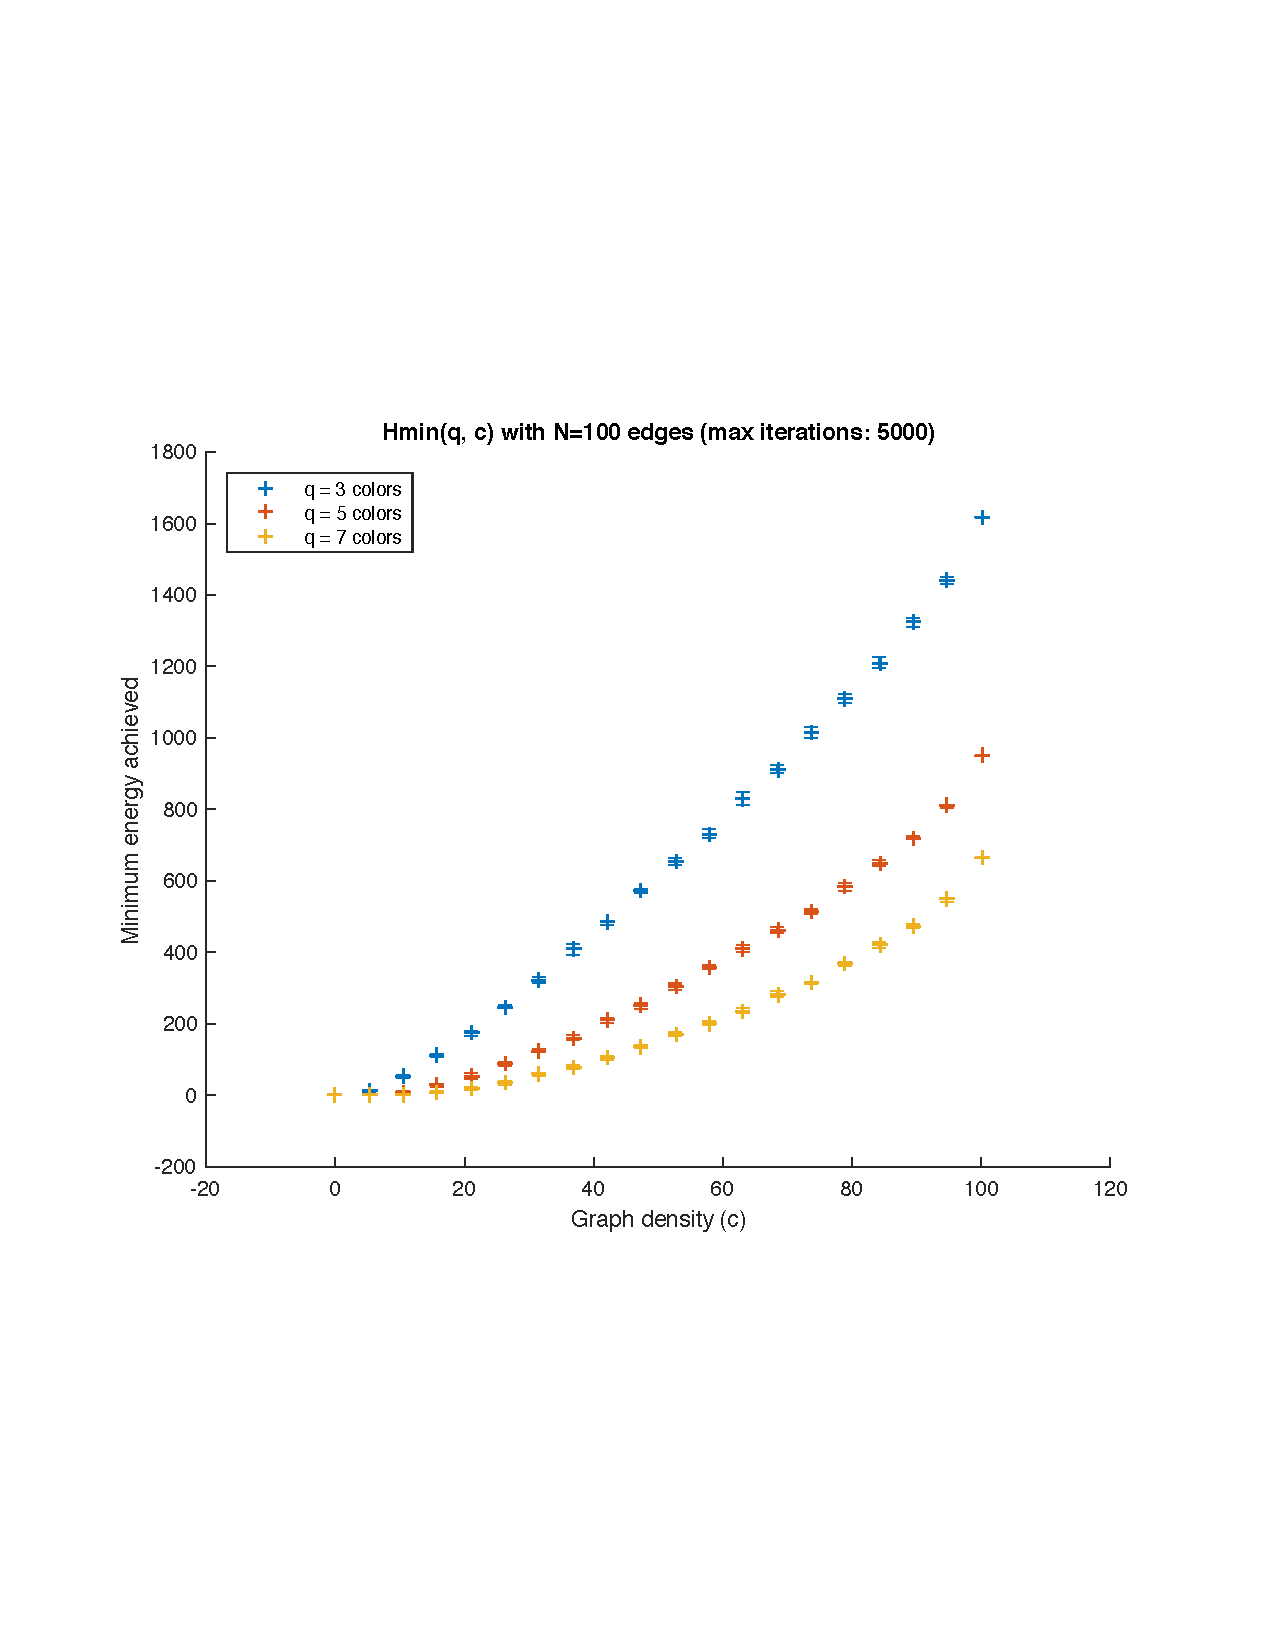
\includegraphics[width=8cm]{figures/cost-vs-graph-density.pdf}
    \end{center}
    \label{Fig:cost-vs-density}
    \caption{Minimal energy achieved as a function of graph density for different values of $q$. Since both the input data and the process are random, we perform the optimization for 5 inputs for each set of parameters and show error bars.}
  \end{figure}

\end{document}

